% Some help here: https://en.wikibooks.org/wiki/LaTeX/Document_Structure

% Preamble
% ---
\documentclass{report}

\usepackage[left=0.5in,right=0.5in,bottom=0.5in,top=0.5in]{geometry}

% Packages
% ---
\usepackage{graphicx} % Add pictures to your document
\graphicspath{ {images/} }  % we will keep our images organized under the images directory
\usepackage{listings} % Source code formatting and highlighting
\usepackage{xcolor}   % needed to color hyperlinks and source code
\usepackage{hyperref} % create hyperlinks
\usepackage[T1]{fontenc} % make sure quotes in Python listings are straight quotes
\usepackage{tcolorbox}
\usepackage{siunitx} % Allows us to use math symbols (like Omega) in normal paragraphs
\usepackage{float} % Allows specifying putting an image exactly where it is in the .tex code flow
\usepackage{tikz} % draw diagrams (like the resistor color bands) directly in the document
\usepackage{multicol} % lay out short lists (like the components list) in columns
\usepackage{enumitem} % control the spacing of list items
\usepackage{pdfpages} % used to include an externally created PDF (like our cover)
\usepackage{titlesec} % allow formatting of the chapter/section headers

% formatting of chapters shamelessly copied from here: https://tex.stackexchange.com/a/591399
%%%%%%%%%% chapters
\titleformat
{\chapter} % command to format
[block] % shape: hang, display, block, frame etc
{\sffamily\bfseries\Large}  % format of label + chapter title
{\chaptertitlename\ \thechapter:} % label "Chapter 1:"
{1.5ex} % separation label - chapter title
{} % code before

\titlespacing{\chapter}
{0pt} %left of the label + title
{*0} % vertical space before the title
{*6.5} % idem after title (in ex units + glue)

%%%%%%%%%%%%%%  sections
\titleformat{\section}
[block] % shape
{\sffamily\large\bfseries}% format (keep the chapter font family!)
{\thesection} % label "1.1"
{0.8ex}% separation label -  section title
{}

\titlespacing{\section}
{0pt} %left of label + section title
{*4} % before the label + section title
{*1.5} % after

\titleformat{\subsection}
[block] % shape
{\sffamily\bfseries}% format (keep the chapter font family!)
{\thesubsection} % label "1.1.1"
{0.8ex}% separation label -  section title
{}

\titlespacing{\subsection}
{0pt} %left of label + section title
{*4} % before the label + section title
{*1.5} % after

\hypersetup{
    linktoc=all,              % set to all if you want both sections and subsections linked
    colorlinks=false,         % hyperlink text will be black
    linkbordercolor=black,    % hyperlink borders will be black
    pdfborderstyle={/S/U/W 1} % border style will be underline of width 1pt
}

\lstloadlanguages{Python}
\lstset{
  language=Python,
  numberstyle=\color{gray},
  stringstyle=\color[HTML]{933797},
  commentstyle=\color[HTML]{228B22},
  emph={[2]from,import,pass,return}, emphstyle={[2]\color[HTML]{DD52F0}},
  emph={[3]range}, emphstyle={[3]\color[HTML]{D17032}},
  emph={[4]for,in,def}, emphstyle={[4]\color{blue}},
  showstringspaces=false,
  breaklines=true,
  prebreak=\mbox{{\color{gray}\tiny$\searrow$}},
  numbers=left,
  xleftmargin=15pt,
}

% Helper: include an image if the file exists, otherwise show a placeholder box
\newcommand{\maybeincludegraphics}[2][]{%
  \IfFileExists{images/#2}{%
    \includegraphics[#1]{#2}%
  }{%
    \framebox[0.6\linewidth][c]{\textit{[photo placeholder]}}%
  }%
}

% The parts list at the top of every project. Two tight columns keep it to a
% few lines instead of a long ladder of mostly empty page.
\setlength{\multicolsep}{6pt plus 2pt minus 1pt}
% The interline penalty keeps a wrapped item from being split across the two
% columns, which would leave its tail sitting in the second column with no bullet.
\newenvironment{components}
  {\begin{multicols}{2}\interlinepenalty=10000\begin{itemize}[nosep, leftmargin=1.3em]}
  {\end{itemize}\end{multicols}}

% Breadboard coordinates. \bbhole defines a named coordinate at its first use
% and prints it in bold; \bbref prints that same coordinate again later. The
% diagram generator reads only the \bbhole definitions from the project text.
\newcommand{\bbhole}[2]{%
  \expandafter\gdef\csname bbhole@#1\endcsname{#2}%
  \textbf{#2}%
}
\newcommand{\bbref}[1]{%
  \ifcsname bbhole@#1\endcsname
    \textbf{\csname bbhole@#1\endcsname}%
  \else
    \PackageError{project-guide}{Undefined breadboard hole `#1'}%
      {Define it first with \string\bbhole\string{#1\string}\string{coordinate\string}.}%
  \fi
}

% A machine-readable wiring row and its two breadboard endpoints. The first
% argument is a stable connection name. The remaining arguments print the
% peripheral pin, XIAO pin, and jumper holes while also defining those holes
% for later \bbref uses. The diagram generator reads the same five arguments.
\newcommand{\connectionrow}[5]{%
  \expandafter\gdef\csname bbhole@jumper.#1.start\endcsname{#4}%
  \expandafter\gdef\csname bbhole@jumper.#1.end\endcsname{#5}%
  #2 & #3 & \textbf{#4} $\rightarrow$ \textbf{#5} \\
}

\begin{document}

% Include the title page PDF if it exists; skip gracefully during CI when not yet present
\IfFileExists{title_page.pdf}{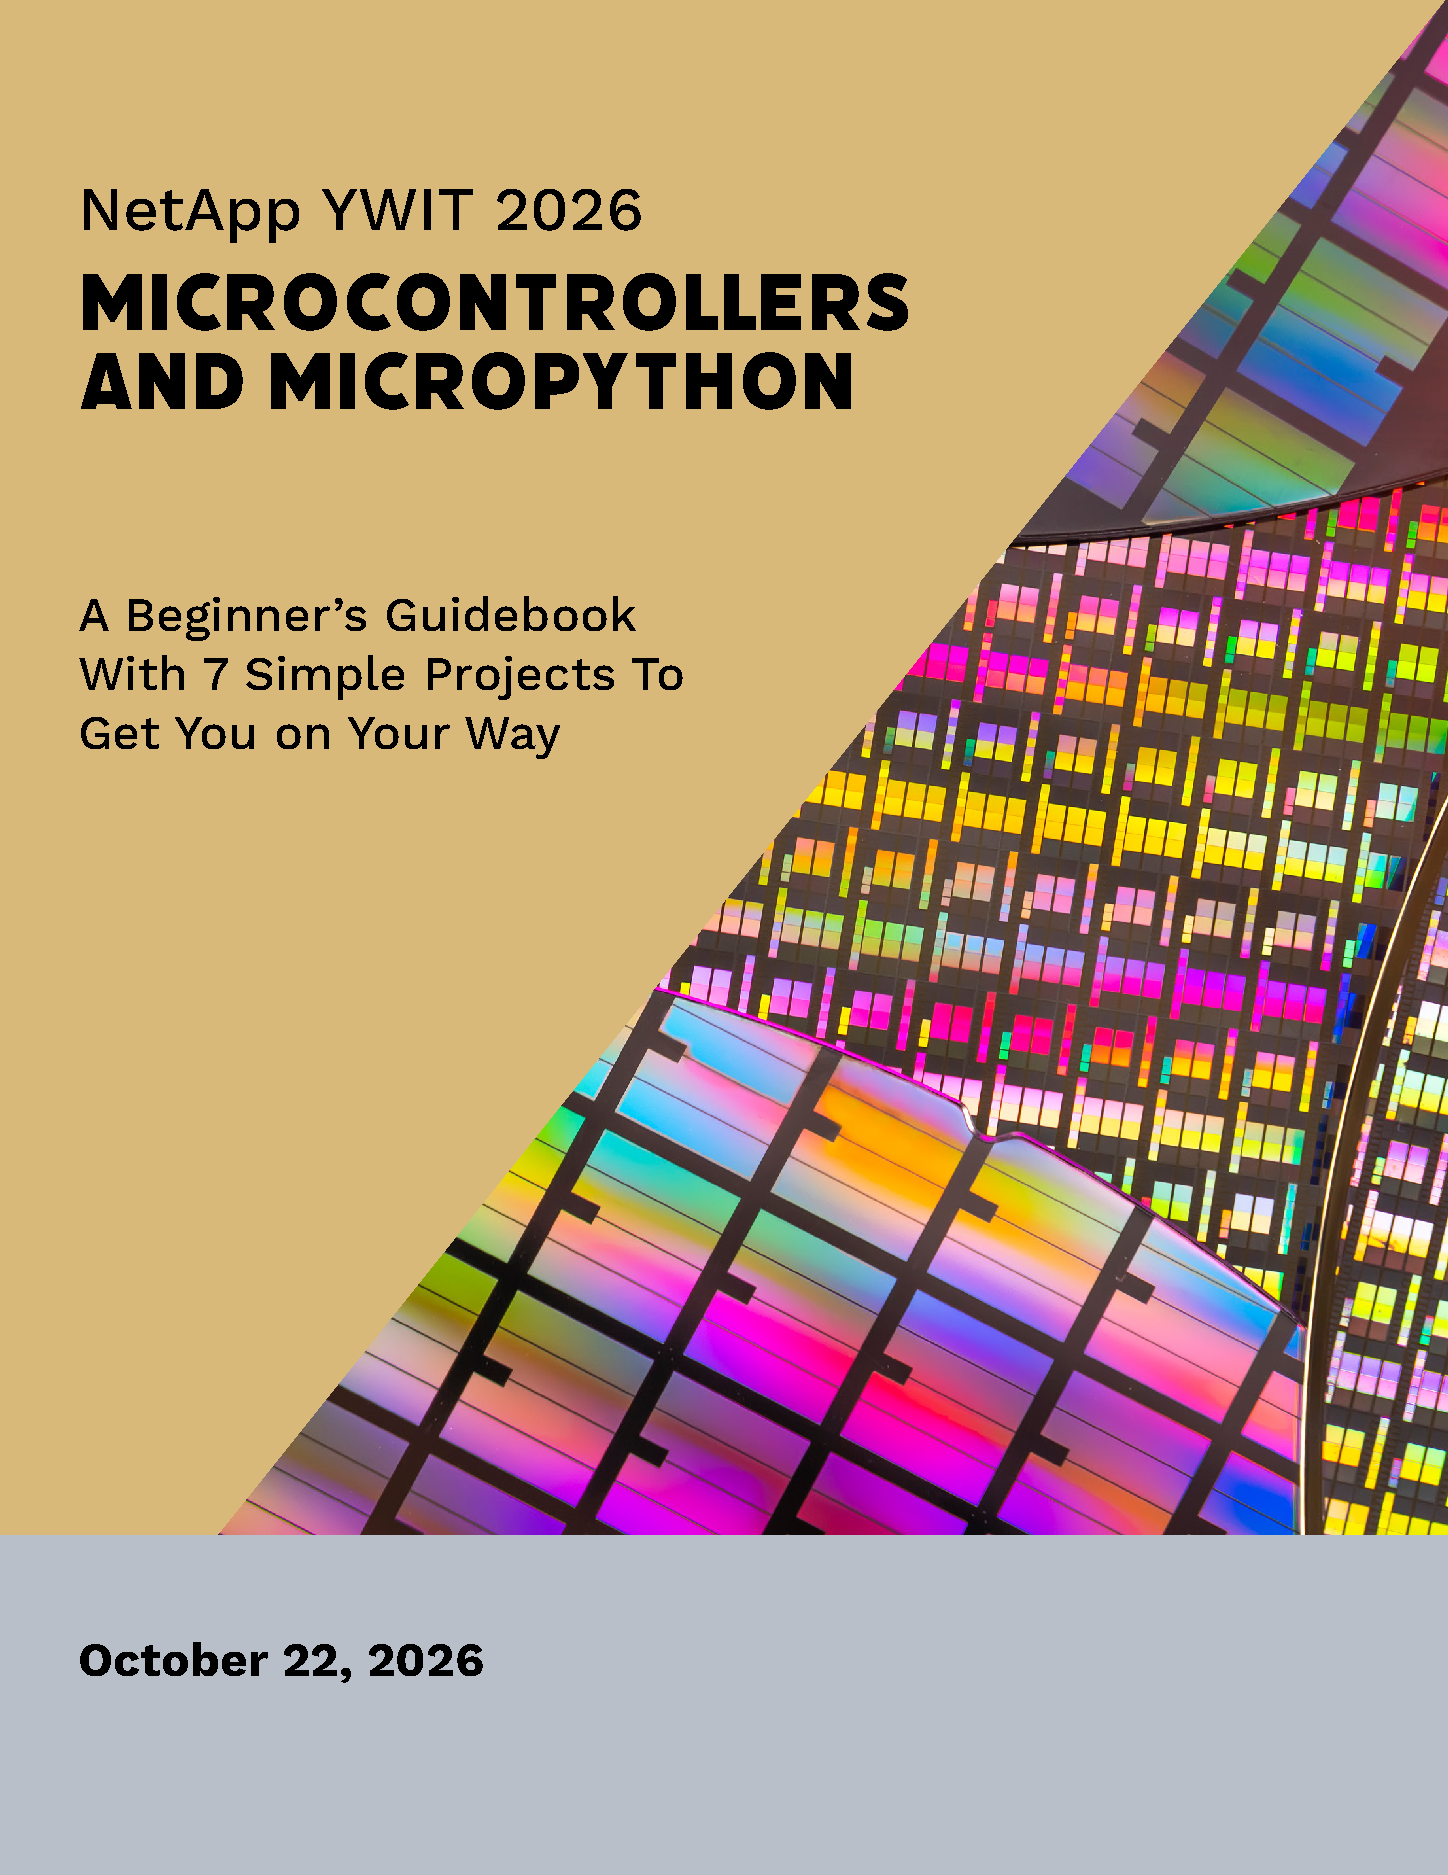
\includepdf{title_page.pdf}}{}

\tableofcontents

\input{introduction/introduction.tex}
\chapter{Electronics Essentials} \label{electronics_essentials}

This beginner's guide introduces the essential components and circuit-building concepts
you will use throughout this workshop. We will cover the breadboard, LEDs, current-limiting
resistors, pushbuttons, jumper wires, and fundamental electrical safety. Later projects will
introduce additional modules---such as addressable RGB LEDs, rotary encoders, speakers, OLED
displays, and motion sensors---which connect using these same breadboard rows and power rails.

\section{The Breadboard: Your Circuit's Foundation}

\subsection{What is a breadboard?}
A breadboard is a reusable platform for prototyping electronic circuits without soldering.
It contains a grid of spring-clip holes into which component leads and jumper wires are
inserted to make electrical connections.

\begin{figure}[H]
    \centering
    \maybeincludegraphics[width=.85\linewidth]{electronics_preamble/breadboard_illustration.png}
    \caption{The workshop breadboard with the Seeed XIAO ESP32-C3 microcontroller seated.}
    \label{fig:breadboard_overview}
\end{figure}

\subsection{Understanding the layout}

\subsubsection{Numbered columns (Bus Strips)}
The main area of the breadboard is divided into lettered rows (labeled A through J) and numbered
columns (labeled 1 to 30):
\begin{itemize}
    \item On the bottom half, holes \textbf{A}, \textbf{B}, \textbf{C}, \textbf{D}, and \textbf{E} in the
    \textbf{same numbered column} are connected together internally by a vertical metal clip (a \textit{bus strip}).
    For example, placing two component leads in \textbf{A10} and \textbf{C10} connects them together because both
    share column 10.
    \item On the top half, holes \textbf{F}, \textbf{G}, \textbf{H}, \textbf{I}, and \textbf{J} in the
    \textbf{same numbered column} are likewise connected together.
    \item \textbf{Adjacent column numbers are NOT connected.} Column 10 is completely separate from Column 11.
\end{itemize}

\subsubsection{The center divider}
A plastic trench separates rows A--E from rows F--J. The two sides are \textbf{electrically isolated}
unless you connect a jumper wire across the gap. The microcontroller straddles this center trench so that
its bottom pins (in row D) and top pins (in row H) connect to separate 5-hole bus strips.

\subsubsection{Power rails}
Along the top and bottom edges run long horizontal strips called \textbf{power rails}:
\begin{itemize}
    \item \textbf{Positive rail (+, red line):} Used to distribute power (3.3V) across the board.
    \item \textbf{Ground rail (--, blue line):} Used as the common ground (GND) return path.
\end{itemize}
All holes along the same rail are connected horizontally across all columns. Once your microcontroller is seated, you
will run jumper wires from its \textbf{3V3} and \textbf{GND} pins to these rails to power your circuits.

\begin{tcolorbox}[colback=blue!5!white,colframe=blue!40!black]
    \textbf{Breadboard summary:} Holes in the \textbf{same numbered column} on the \textbf{same side} of the
    center divider (e.g., A10 through E10) are connected together. Holes in different numbered columns, or on
    opposite sides of the center divider, are separated until you connect them with a component or jumper wire.
\end{tcolorbox}


\section{LEDs: Lighting Up Your Circuits}

\subsection{What is an LED?}
An LED (Light-Emitting Diode) is a semiconductor device that produces light when electric current flows
through it in the correct direction.

\subsection{Polarity}
LEDs are \textbf{polarized}---electricity can only flow through them in one direction:
\begin{itemize}
    \item \textbf{Anode (+):} The longer leg. Connects toward the positive voltage source (microcontroller GPIO pin).
    \item \textbf{Cathode (--):} The shorter leg. Connects toward Ground (GND). If the legs have been trimmed, look for the \textbf{flat edge} on the plastic rim of the LED casing on the cathode side.
\end{itemize}

\begin{figure}[H]
\centering
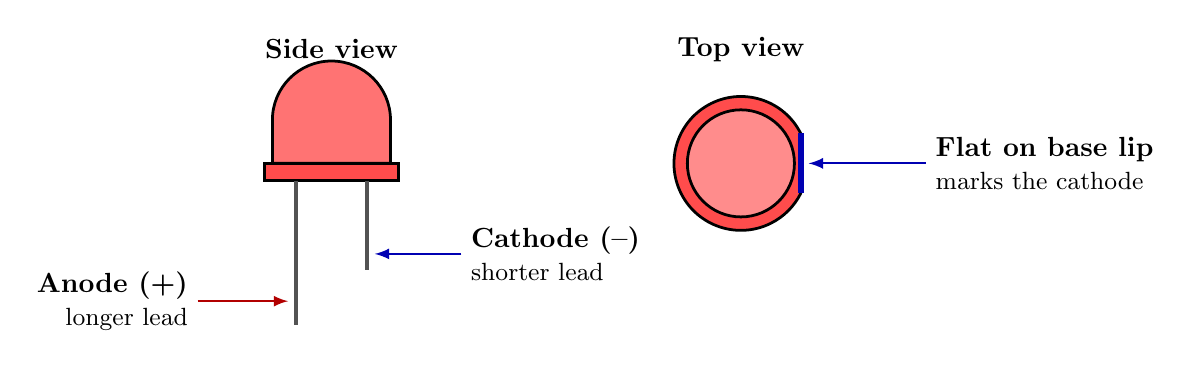
\begin{tikzpicture}[x=1cm,y=1cm,>=latex]
    % Side view: the unequal lead lengths are deliberately exaggerated.
    \node[font=\bfseries] at (-2.2,1.45) {Side view};
    \fill[red!55,draw=black,line width=1pt]
        (-2.95,0) -- (-2.95,0.55) arc[start angle=180,end angle=0,radius=0.75]
        -- (-1.45,0) -- cycle;
    \fill[red!70,draw=black,line width=1pt] (-3.05,-0.22) rectangle (-1.35,0);
    \draw[line width=1.6pt,gray!65!black] (-2.65,-0.22) -- (-2.65,-2.05);
    \draw[line width=1.6pt,gray!65!black] (-1.75,-0.22) -- (-1.75,-1.35);

    \draw[->,thick,red!70!black] (-3.9,-1.75) -- (-2.75,-1.75);
    \node[anchor=east,align=right] at (-3.9,-1.75)
        {\textbf{Anode (+)}\\\small longer lead};
    \draw[->,thick,blue!70!black] (-0.55,-1.15) -- (-1.65,-1.15);
    \node[anchor=west,align=left] at (-0.55,-1.15)
        {\textbf{Cathode (--) }\\\small shorter lead};

    % Top view: the dome is round; only the wider base lip has a small flat.
    \node[font=\bfseries] at (3.0,1.45) {Top view};
    \fill[red!70,draw=black,line width=1pt]
        (3.76,0.38)
        arc[start angle=26.6,end angle=333.4,radius=0.85]
        -- cycle;
    \fill[red!45,draw=black,line width=1pt] (3.0,0) circle[radius=0.68];
    \draw[line width=2pt,blue!70!black] (3.76,-0.38) -- (3.76,0.38);
    \draw[->,thick,blue!70!black] (5.35,0) -- (3.86,0);
    \node[anchor=west,align=left] at (5.35,0)
        {\textbf{Flat on base lip}\\\small marks the cathode};
\end{tikzpicture}
\caption{Use either clue to identify LED polarity: the cathode has the shorter lead and the flat edge.}
\label{fig:led_polarity}
\end{figure}

\subsection{Current-limiting resistor}
LEDs have very little internal resistance. If connected directly between power and ground, too much current
will flow, destroying the LED and potentially damaging the microcontroller pin.

You must \textbf{always connect a resistor in series} with an LED. ``In series'' means the current must travel
through one single path: from the pin, through the LED, through the resistor, and into ground (or vice versa).
In this kit, we use a \textbf{220\si{\ohm}} resistor for the LED.


\section{Resistors: Controlling Current Flow}

\subsection{What is a resistor?}
A resistor is a passive component that resists and limits the flow of electric current. Resistors protect
sensitive components (like LEDs) and help create reference voltages for analog sensors. Resistors have
\textbf{no polarity}---they can be installed in either orientation without affecting the circuit.

\subsection{Resistance values and identification}
Resistance is measured in ohms (\si{\ohm}) and kilohms (\SI{1}{\kilo\ohm} = \SI{1000}{\ohm}). The resistance
value is indicated by colored bands around the body of the resistor.

% Telling the 220 ohm and 10k ohm resistors apart. The resistors are drawn with
% TikZ rather than photographed because the band colors have to stay readable
% when the guide is printed in a classroom.
\definecolor{bodymetal}{HTML}{9FC2E8}
% xcolor's brown is a light tan that reads as gold next to the other bands.
\definecolor{bandbrown}{HTML}{7B4A12}

% \resistorglyph{band 1}{band 2}{band 3}{band 4}{band 5}
% The kit's resistors carry one band on each end bulge and three across the
% middle, all at roughly even spacing, so the geometry here is fixed.
\newcommand{\resistorglyph}[5]{%
\begin{tikzpicture}[x=1cm, y=1cm]
    \draw[line width=1pt, gray!50!black] (-0.5,0.3) -- (2.8,0.3);
    \draw[fill=bodymetal, draw=black!55] (0.24,0.04) rectangle (2.06,0.56);
    \draw[fill=bodymetal, draw=black!55, rounded corners=3pt] (0.02,0) rectangle (0.46,0.6);
    \draw[fill=bodymetal, draw=black!55, rounded corners=3pt] (1.84,0) rectangle (2.28,0.6);
    \fill[#1] (0.16,0.01) rectangle (0.32,0.59);
    \fill[#2] (0.62,0.05) rectangle (0.78,0.55);
    \fill[#3] (1.07,0.05) rectangle (1.23,0.55);
    \fill[#4] (1.52,0.05) rectangle (1.68,0.55);
    \fill[#5] (1.98,0.01) rectangle (2.14,0.59);
\end{tikzpicture}%
}

% \resistorcell{value}{band 1}{band 2}{band 3}{band 4}{band 5}{caption}
\newcommand{\resistorcell}[7]{%
\begin{tabular}{c}
    \textbf{#1} \\[4pt]
    \resistorglyph{#2}{#3}{#4}{#5}{#6} \\[2pt]
    \small #7
\end{tabular}%
}

\begin{tcolorbox}[colback=yellow!10!white,colframe=yellow!50!black]
    \textbf{Which resistor is which?} Both resistors are small and blue with five evenly spaced
    colored bands, and nothing is printed on them. You do not need to figure out which end to read
    from---just count the \textbf{red} bands. The \textbf{220\si{\ohm}} resistor has \textbf{two red
    bands next to each other}, and the \textbf{10\si{\kilo\ohm}} resistor has \textbf{exactly one red
    band}. Swapping the two will not damage anything, but the circuit will not behave the way this
    project describes, so ask an instructor if you are not sure.

    \medskip
    \centering
    \begin{tabular}{c @{\hspace{3em}} c}
        \resistorcell{220\si{\ohm}}{red}{red}{black}{black}{bandbrown}{two red bands} &
        \resistorcell{10\si{\kilo\ohm}}{bandbrown}{black}{black}{red}{bandbrown}{one red band}
    \end{tabular}
\end{tcolorbox}



\section{Buttons: User Input} \label{button_basics}

\subsection{What is a pushbutton?}
A pushbutton is a momentary switch that completes a connection when pressed and breaks it when released.
The buttons in your kit have four pins arranged in two connected pairs.

\begin{figure}[H]
\centering
    \maybeincludegraphics[width=.8\linewidth]{electronics_preamble/button_illustration.png}
    \caption{Pushbutton pin arrangement: the two pins on each side are internally joined.}
    \label{fig:button_pinout}
\end{figure}

\subsection{Understanding the 4-pin connection}
As shown in Figure \ref{fig:button_pinout}, the two pins on the top edge are permanently joined internally,
and the two pins on the bottom edge are permanently joined internally. Pressing the button bridges the gap
between the top pair and the bottom pair. When placing the button across rows on the breadboard, ensure your
two circuit connections go to opposite pairs so pressing the button closes the circuit.

\subsection{Internal pull-up resistors}
When a button is not pressed, an input pin would otherwise be left ``floating'' (unconnected), picking up
electrical noise. The ESP32-C3 microcontroller has built-in \textbf{pull-up resistors} that can be enabled
in MicroPython code. This pulls the pin HIGH (3.3V) when idle; pressing the button connects the pin to GND,
pulling it LOW (0V). This means you do not need an external resistor to wire a button!

Although both components are called resistors, an internal pull-up cannot replace the
220\si{\ohm} current-limiting resistor used with an LED. A pull-up is a weak, relatively
high-value resistor (typically tens of kilohms) connected inside the microcontroller between
3.3V and an \textbf{input} pin. Its job is only to keep an otherwise unconnected input at a
known logic level. It is not in the LED's current path, its exact value is not tightly
controlled, and it would supply far too little current to light the LED normally. The external
220\si{\ohm} resistor has a known value and is physically placed \textbf{in series} with the
LED so that all LED current passes through it.


\section{Jumper Wires: Making Connections}

\subsection{What are jumper wires?}
Jumper wires are flexible insulated wires with male pins at both ends that plug directly into breadboard holes.

\begin{figure}[H]
\centering
    \maybeincludegraphics[width=.7\linewidth]{electronics_preamble/jumper_illustration.png}
    \caption{Male-to-male jumper wires in various colors.}
    \label{fig:jumper_wires}
\end{figure}

\subsection{Wire colors}
All jumper wires are electrically identical on the inside. However, following standard color conventions
makes your circuits much easier to read and troubleshoot:
\begin{itemize}
    \item \textbf{Red / Orange:} Positive power supply (+3.3V or 5V).
    \item \textbf{Black:} Ground (GND).
    \item \textbf{Yellow / Green / Blue / Purple:} Signals and data lines (GPIO pins).
\end{itemize}


\section{Safety Guidelines}

Working with 3.3V microcontroller circuits is safe and will not deliver an electric shock, but observing
a few basic rules will protect your components from damage:

\begin{itemize}
    \item \textbf{Unplug before rewiring:} Always disconnect the USB cable from your computer before placing
    or moving components on the breadboard.
    \item \textbf{Avoid short circuits:} Never connect a jumper wire directly from the positive rail (3.3V or 5V)
    to the ground rail (GND). This causes a short circuit that can overheat the board.
    \item \textbf{Always use a series resistor with LEDs:} Directly connecting an LED between 3.3V and GND
    without a 220\si{\ohm} resistor will burn out the LED.
    \item \textbf{3.3V logic levels:} The ESP32-C3 GPIO pins operate at 3.3V. Always power modules in this kit
    from the 3.3V pin unless a specific project instructs otherwise.
    \item \textbf{Disconnect if hot:} If any component feels hot to the touch or you notice a burning smell,
    immediately unplug the USB cable and ask an instructor to inspect your wiring.
\end{itemize}

\input{micropython_ide/micropython_ide.tex}

\chapter{Project 1: Blink}

\section{Overview}
% TODO: Fill in project overview
This project is a placeholder for Project 1.

\pagebreak

\section{Directions}

\subsection{Creating the circuit}
% TODO: Add wiring instructions and breadboard diagram

\subsection{Programming the microcontroller}
% TODO: Add programming instructions
Click on the file named "project\_1\_blink.py" and run it using the IDE.
Refer back to Chapter \ref{ide} for IDE instructions.

\section{Review}
% TODO: Add review content

\section{Possible Extensions}
% TODO: Add extension ideas

\chapter{Project 2: Red Light, Green Light}

\section{Overview}
In this project, you will build a reflex game with a button and a 3-pixel WS2812B LED strip.
Each reaction window cycles through red, yellow, and green phases:
\begin{itemize}
    \item During \textbf{RED}, do not press. Pressing during red ends the round immediately.
    \item During \textbf{YELLOW}, get ready for green and do not press yet.
    \item During \textbf{GREEN}, press the button as quickly as possible to score a point.
\end{itemize}

Each successful green press prints your reaction time in milliseconds to the serial console.
Each round has 5 total reaction windows. A hit during green scores a point, and a missed green
window counts as a miss.

\begin{tcolorbox}[colback=blue!5!white,colframe=blue!40!black]
    \textbf{Learning goals:}
    \begin{itemize}
        \item Read a pushbutton using an internal pull-up resistor
        \item Control WS2812B addressable LEDs with MicroPython
        \item Build a simple game state machine
        \item Measure reaction time with millisecond timers
    \end{itemize}
\end{tcolorbox}

\pagebreak

\section{Components}
\begin{itemize}
    \item Seeed XIAO ESP32-C3 microcontroller
    \item 3x WS2812B addressable RGB LEDs wired in series
    \item 1x pushbutton
    \item Breadboard
    \item Jumper wires
\end{itemize}

\section{Directions}

\subsubsection{Remove previous components}
Before starting Project 2, remove components and wires from the previous project.

\subsection{Creating the circuit}

\subsubsection{WS2812B strip wiring}
The strip has a right-angle header soldered to its \textbf{DI} end, so it stands upright once
seated. Push those three pins into the top half of the board: \textbf{5V} into
\bbhole{pixels.header.power}{J12}, \textbf{DI} into \bbhole{pixels.header.data}{J13}, and
\textbf{GND} into \bbhole{pixels.header.ground}{J14}. Then add these connections:
\begin{center}
\begin{tabular}{|l|l|l|}
    \hline
    \textbf{WS2812B pin} & \textbf{XIAO pin} & \textbf{Jumper holes} \\
    \hline
    \connectionrow{pixels-power}{5V (power in)}{3V3}{I3}{I12}
    \connectionrow{pixels-data}{DI (first LED)}{GPIO 20}{I7}{I13}
    \connectionrow{pixels-ground}{GND}{GND}{I2}{I14}
    \hline
\end{tabular}
\end{center}

\subsubsection{Button wiring}
Press the button into the bottom edge of the board so that its legs reach from column \textbf{A}
up to column \textbf{D}. One pair of legs goes into \bbhole{button.side-a}{A12} and \textbf{D12},
and the other pair two rows along into \bbhole{button.side-b}{A14} and \textbf{D14}. The two legs
of a pair are already joined inside the button, so it is the gap between the two pairs that the
button closes. Then add these connections:
\begin{center}
\begin{tabular}{|l|l|l|}
    \hline
    \textbf{Button connection} & \textbf{XIAO pin} & \textbf{Jumper holes} \\
    \hline
    \connectionrow{button-signal}{One side}{GPIO 21}{C7}{E12}
    \connectionrow{button-ground}{Other side}{GND}{J2}{E14}
    \hline
\end{tabular}
\end{center}

The code enables the internal pull-up resistor, so the pin reads HIGH when idle and LOW when pressed.

\begin{figure}[H]
    \centering
    \maybeincludegraphics[width=.9\linewidth]{project_2/wiring.png}
    \caption{Connect the LED strip and button to the XIAO ESP32-C3.}
\end{figure}

\subsection{Programming the microcontroller}
Open the file \texttt{project\_2\_red\_light\_green\_light.py} and run it in the IDE (Chapter \ref{ide}).

At startup, the serial console will print instructions and wait for a button press to begin:
\begin{verbatim}
Project 2: Red Light, Green Light
Press button to start.
\end{verbatim}

During gameplay:
\begin{itemize}
    \item The 3 LEDs act like a stoplight: red LED, yellow LED, and green LED are used individually.
    \item RED phase lights only the red LED and prints ``RED! Do not press.''
    \item YELLOW phase lights only the yellow LED and prints ``YELLOW! Get ready...''
    \item GREEN phase lights only the green LED and prints ``GREEN! Press now.''
    \item Idle/round-over uses the yellow LED as a waiting indicator.
    \item A valid green press prints reaction time and increases score.
    \item A missed green window is counted as one of the 5 windows.
    \item A red/yellow press ends the round and prints final score + best reaction.
\end{itemize}

\subsection{Hardware test checklist}
Use this checklist to confirm your circuit and code are working:
\begin{enumerate}
    \item Confirm LED order on your strip: first LED (DI side) is red, middle is yellow, last is green.
    \item Press button from idle state: yellow wait indicator transitions into red/green gameplay cycling.
    \item Wait for GREEN (green LED only) and press quickly: score increases and a reaction time is printed.
    \item Do not press during RED or YELLOW: pressing before green ends the round immediately.
    \item Skip pressing during one green window: verify it is counted as a miss and the next window starts.
    \item Repeat at least 5 rounds to confirm stable behavior and reliable button detection.
\end{enumerate}

\section{Review}
In this project, you combined timed logic, button input, and LED output to build a full game loop.
You practiced:
\begin{itemize}
    \item State-based programming (idle, green, red, round\_over)
    \item Reusing a shared debounced button library for cleaner input handling
    \item Using \texttt{time.ticks\_ms()} and \texttt{time.ticks\_diff()} for timing
    \item Providing immediate visual and text feedback to players
\end{itemize}

\section{Possible Extensions}
Try these enhancements:
\begin{itemize}
    \item Add difficulty levels by shrinking GREEN timing windows
    \item Display average reaction time after each round
    \item Add a buzzer sound effect for valid and invalid presses
    \item Use different LED patterns (chase, blink, gradient) per game state
    \item Add a countdown before each round starts
\end{itemize}

\chapter{Project 3: Reflex Arcade}

\section{Overview}
% TODO: Fill in project overview
This project is a placeholder for Project 3 (Reflex Arcade).
A reaction-time game where an LED lights up after a random delay and the user must press
their button as fast as possible. Their reaction time is calculated and displayed on the screen.

\pagebreak

\section{Directions}

\subsection{Creating the circuit}
% TODO: Add wiring instructions and breadboard diagram

\subsection{Programming the microcontroller}
% TODO: Add programming instructions
Click on the file named "project\_3\_reflex\_arcade.py" and run it using the IDE.
Refer back to Chapter \ref{ide} for IDE instructions.

\section{Review}
% TODO: Add review content

\section{Possible Extensions}
% TODO: Add extension ideas

\chapter{Project 4: Pocket DJ}

\section{Overview}
In this project, you will turn your microcontroller into a handheld musical instrument: the \textbf{Pocket DJ}!
You will wire three pushbuttons, a mini speaker, and a 3-pixel RGB LED strip to your breadboard.
Pressing each button triggers a distinct musical note on the speaker and lights up a matching colored pixel on the LED strip.

Over the course of this project, you will:
\begin{itemize}
    \item Connect multiple tactile pushbuttons and read them using MicroPython
    \item Use PWM (Pulse Width Modulation) to generate different pitch frequencies on a speaker
    \item Control individual addressable WS2812B RGB LEDs to create synchronized visual pulses
    \item Program rhythm loops and sound sequences using Python lists and tuples
\end{itemize}

\begin{figure}[H]
\centering
    \maybeincludegraphics[width=.6\linewidth]{project_4/success.jpg}
    \caption{The assembled Pocket DJ ready to drop some beats!}
\end{figure}

\begin{tcolorbox}[colback=blue!5!white,colframe=blue!40!black]
    \textbf{Learning goals:}
    \begin{itemize}
        \item Read pushbuttons with active-low logic and internal pull-up resistors
        \item Generate musical notes by controlling PWM frequency on a speaker
        \item Control WS2812B addressable LEDs using the \texttt{neopixel} library
        \item Structure musical sequences and automated rhythm loops in code
    \end{itemize}
\end{tcolorbox}

\pagebreak

\section{Components}
\begin{components}
    \item Seeed XIAO ESP32-C3 microcontroller
    \item 3-pixel WS2812B LED strip
    \item 3x Tactile pushbuttons ($6\times6$\,mm)
    \item 1x Treedix 1W 8\si{\ohm} mini speaker (with breadboard-friendly Dupont leads)
    \item Breadboard
    \item Jumper wires
\end{components}

\section{Directions}

\subsubsection{Remove previous components}
Before beginning, remove components and wires from the previous project. You may leave the
microcontroller seated in the breadboard.

\subsection{Creating the circuit}

% Seating the microcontroller. This is identical for every project, so the
% coordinates live here rather than in any one project chapter. The diagram
% generator reads the \bbhole definitions below for every breadboard diagram
% it draws, which is why this file is the only place they appear.
\subsubsection{Attach the microcontroller to the breadboard}
Orient the microcontroller so that the pin labeled \textbf{5V} goes into hole \bbhole{mcu.5v}{H1}
(Column H, Row 1), \textbf{GPIO2} into \bbhole{mcu.gpio2}{D1}, \textbf{GPIO20} into
\bbhole{mcu.gpio20}{H7}, and \textbf{GPIO21} into \bbhole{mcu.gpio21}{D7}. Then press it down---this
takes more force than you might expect.

\begin{figure}[H]
    \centering
    \maybeincludegraphics[width=.95\linewidth]{common/microcontroller_seated_in_breadboard.png}
    \caption{So far, so good!}
\end{figure}


\subsubsection{Ground rail distribution}
Because we have multiple components requiring a ground connection, we connect the microcontroller's
\textbf{GND} pin to the breadboard's top blue ($-$) power rail. This powers the entire rail with ground:

\begin{center}
\begin{tabular}{|l|l|l|}
    \hline
    \textbf{Connection} & \textbf{XIAO pin} & \textbf{Jumper holes} \\
    \hline
    \connectionrow{mcu-ground}{Top GND rail}{GND}{I2}{top-2}
    \hline
\end{tabular}
\end{center}

\subsubsection{WS2812B LED strip placement and wiring}
The LED strip has a right-angle header so it stands upright once seated.
Insert those three pins into row \textbf{F} (rows 22--24) on the right side of the breadboard so it is
clearly visible and not obscured by jumper wires:
\textbf{5V} into \bbhole{pixels.header.power}{F22},
\textbf{DI} into \bbhole{pixels.header.data}{F23}, and
\textbf{GND} into \bbhole{pixels.header.ground}{F24}.
Then connect the jumper wires:

\begin{center}
\begin{tabular}{|l|l|l|}
    \hline
    \textbf{WS2812B pin} & \textbf{Source / Pin} & \textbf{Jumper holes} \\
    \hline
    \connectionrow{pixels-power}{5V}{3V3}{I3}{J22}
    \connectionrow{pixels-data}{DI}{GPIO 20}{I7}{J23}
    WS2812B ground & Top GND rail & \bbhole{jumper.pixels-ground.start}{top-24} $\rightarrow$ \bbhole{jumper.pixels-ground.end}{J24} \\
    \hline
\end{tabular}
\end{center}

\subsubsection{Tactile button placement and wiring}
Seat the three pushbuttons in the lower half of the breadboard spanning columns \textbf{A} through \textbf{D}:
\begin{itemize}
    \item \textbf{Pad 0 (Loop/Bass):} Place one pair of legs in \bbhole{pad0.side-a}{A10} and \textbf{D10}, and the other pair in \bbhole{pad0.side-b}{A12} and \textbf{D12}.
    \item \textbf{Pad 1 (Mid note):} Place one pair of legs in \bbhole{pad1.side-a}{A14} and \textbf{D14}, and the other pair in \bbhole{pad1.side-b}{A16} and \textbf{D16}.
    \item \textbf{Pad 2 (High note):} Place one pair of legs in \bbhole{pad2.side-a}{A18} and \textbf{D18}, and the other pair in \bbhole{pad2.side-b}{A20} and \textbf{D20}.
\end{itemize}

Connect each button's signal leg (column \textbf{E}) to the microcontroller:
\begin{center}
\begin{tabular}{|l|l|l|}
    \hline
    \textbf{Button signal} & \textbf{XIAO pin} & \textbf{Jumper holes} \\
    \hline
    \connectionrow{pad0-signal}{Pad 0 (row 10)}{GPIO 21}{C7}{E10}
    \connectionrow{pad1-signal}{Pad 1 (row 14)}{GPIO 7}{C6}{E14}
    \connectionrow{pad2-signal}{Pad 2 (row 18)}{GPIO 6}{C5}{E18}
    \hline
\end{tabular}
\end{center}

Next, wire each button's ground leg (column \textbf{E}) to the top ground rail:
\begin{center}
\begin{tabular}{|l|l|l|}
    \hline
    \textbf{Button ground} & \textbf{Source} & \textbf{Jumper holes} \\
    \hline
    Pad 0 ground & Top GND rail & \bbhole{jumper.pad0-ground.start}{top-12} $\rightarrow$ \bbhole{jumper.pad0-ground.end}{E12} \\
    Pad 1 ground & Top GND rail & \bbhole{jumper.pad1-ground.start}{top-16} $\rightarrow$ \bbhole{jumper.pad1-ground.end}{E16} \\
    Pad 2 ground & Top GND rail & \bbhole{jumper.pad2-ground.start}{top-20} $\rightarrow$ \bbhole{jumper.pad2-ground.end}{E20} \\
    \hline
\end{tabular}
\end{center}

\subsubsection{Speaker placement and wiring}
Insert the speaker's two Dupont leads into the lower half of the breadboard:
the positive red lead into \bbhole{speaker.lead.signal}{C26} and the negative black lead into \bbhole{speaker.lead.ground}{C28}.
Then connect the speaker signal and ground jumpers:

\begin{center}
\begin{tabular}{|l|l|l|}
    \hline
    \textbf{Speaker lead} & \textbf{Source / Pin} & \textbf{Jumper holes} \\
    \hline
    \connectionrow{speaker-signal}{Signal (+)}{GPIO 10}{I4}{E26}
    Speaker ground ($-$) & Top GND rail & \bbhole{jumper.speaker-ground.start}{top-28} $\rightarrow$ \bbhole{jumper.speaker-ground.end}{E28} \\
    \hline
\end{tabular}
\end{center}

\begin{figure}[H]
    \centering
    \maybeincludegraphics[width=.95\linewidth]{project_4/wiring.png}
    \caption{Complete wiring diagram for Project 4: Pocket DJ.}
\end{figure}

\subsection{Programming the microcontroller}
Open the file named \texttt{project\_4\_pocket\_dj.py} in the IDE and run it.

When the script starts, the serial console displays:
\begin{verbatim}
Project 4: Pocket DJ
Pad 0: GPIO 21 | Pad 1: GPIO 7 | Pad 2: GPIO 6
Speaker: GPIO 10 | LED Strip: GPIO 20
Press any button to play music!
\end{verbatim}

Try pressing each pad:
\begin{itemize}
    \item \textbf{Pad 1} plays a middle note (330\,Hz) and flashes the middle LED green.
    \item \textbf{Pad 2} plays a higher note (392\,Hz) and flashes the third LED blue.
    \item \textbf{Pad 0} plays an automated 4-step rhythm loop across the notes and colors!
\end{itemize}

\subsection{How the program works}

\subsubsection{Musical tones with PWM}
In Project 1, PWM was used to control LED brightness by changing duty cycle at a fixed frequency.
Here, we use PWM on the speaker pin, but instead of changing brightness, we change the \textbf{frequency} (the pitch):
\begin{lstlisting}[language=Python, caption=Playing a tone on the speaker]
pwm = PWM(Pin(PIN_SPEAKER), freq=freq, duty=512)
time.sleep_ms(duration_ms)
pwm.deinit()
\end{lstlisting}
A higher frequency makes the speaker vibrate faster, producing a higher musical pitch. A 50\% duty cycle (\texttt{duty=512}) provides optimal volume. Calling \texttt{pwm.deinit()} silences the speaker when the note is done.

\subsubsection{RGB LEDs with NeoPixel}
The WS2812B LEDs are addressable: a single digital data pin (GPIO 20) controls the color and brightness of all three pixels independently.
Colors are specified as \texttt{(Red, Green, Blue)} tuples from 0 to 255:
\begin{lstlisting}[language=Python, caption=Lighting a pixel]
pixels[pixel_idx] = color
pixels.write()
\end{lstlisting}

\subsubsection{Rhythm loops}
Pad 0 reads a sequence of note indices and timing delays stored in a Python tuple:
\begin{lstlisting}[language=Python, caption=Rhythm loop sequence]
LOOP = (
    (0, 80),   # Pad 0, rest 80 ms
    (2, 60),   # Pad 2, rest 60 ms
    (1, 80),   # Pad 1, rest 80 ms
    (2, 120),  # Pad 2, rest 120 ms
)
\end{lstlisting}
When triggered, a \texttt{for} loop steps through each element, playing each note and waiting before the next beat.

\subsection{Hardware test checklist}
\begin{enumerate}
    \item Press Pad 1: You should hear a tone and see the green LED light up.
    \item Press Pad 2: You should hear a higher tone and see the blue LED light up.
    \item Press Pad 0: You should hear the 4-step beat loop play across the different tones and LEDs.
    \item Check serial output in the IDE to verify that button presses are detected cleanly without double triggers.
\end{enumerate}

\begin{tcolorbox}[colback=yellow!10!white,colframe=yellow!50!black]
    \textbf{If something does not work:}
    \begin{itemize}
        \item \textbf{No sound from speaker:} Check that the speaker red lead is in \bbref{speaker.lead.signal} and jumpered from \bbref{jumper.speaker-signal.start} to \bbref{jumper.speaker-signal.end} (GPIO 10). Check that the black lead is in \bbref{speaker.lead.ground} and grounded to the top rail via \bbref{jumper.speaker-ground.start} to \bbref{jumper.speaker-ground.end}.
        \item \textbf{LED strip does not light:} Check that the strip is seated in F22--F24 with DI in \bbref{pixels.header.data} and connected to GPIO 20 (\bbref{jumper.pixels-data.start} to \bbref{jumper.pixels-data.end}), power to 3.3V (\bbref{jumper.pixels-power.start} to \bbref{jumper.pixels-power.end}), and GND to the top rail (\bbref{jumper.pixels-ground.start} to \bbref{jumper.pixels-ground.end}).
        \item \textbf{Button press does nothing:} Verify button orientation and connections. Check that the microcontroller GND wire (\bbref{jumper.mcu-ground.start} to \bbref{jumper.mcu-ground.end}) is connected to the top rail, and each button ground jumper is connected.
    \end{itemize}
\end{tcolorbox}

\section{Review}
In this project, you constructed a multi-component digital instrument combining inputs (pushbuttons) with two different types of outputs (PWM audio on a speaker and addressable RGB LEDs). You learned how frequency determines pitch, how to drive NeoPixel LEDs, and how to program sequenced loops.

\section{Possible Extensions}
\begin{itemize}
    \item \textbf{Custom melodies:} Modify the \texttt{LOOP} tuple in \texttt{project\_4\_pocket\_dj.py} to create your own custom beats or jingles.
    \item \textbf{Scale selector:} Add higher or lower octaves by doubling or halving the frequencies in \texttt{PADS}.
    \item \textbf{DJ light show:} Update \texttt{play\_note} to create visual ripple effects where non-playing LEDs pulse with complementary colors.
\end{itemize}

\chapter{Wi-Fi Mood Lamp}

\section{Overview}
In this project, your ESP32-C3 becomes both a Wi-Fi access point and a light controller.
After uploading a Python file plus one HTML dashboard file, you will connect your phone or
laptop to the microcontroller's network, open a local web page, and control a chain of
three WS2812B LEDs.

You will build:
\begin{itemize}
    \item A password-protected Wi-Fi network hosted by the ESP32-C3
    \item A local web dashboard served directly from the board
    \item Manual lighting controls for all LEDs together and for each LED individually
    \item A set of built-in animations (breathing, rainbow, wipe, and blink)
\end{itemize}

By the end, you will have a complete wireless ``mood lamp'' that works without internet.

\pagebreak

\section{Components}

\begin{components}
    \item Seeed XIAO ESP32-C3 microcontroller
    \item 3-pixel WS2812B LED strip
    \item Breadboard
    \item Jumper wires
\end{components}

\section{Directions}

\subsection{Creating the circuit}
Before starting, remove components from earlier projects that are no longer needed.

% Seating the microcontroller. This is identical for every project, so the
% coordinates live here rather than in any one project chapter. The diagram
% generator reads the \bbhole definitions below for every breadboard diagram
% it draws, which is why this file is the only place they appear.
\subsubsection{Attach the microcontroller to the breadboard}
Orient the microcontroller so that the pin labeled \textbf{5V} goes into hole \bbhole{mcu.5v}{H1}
(Column H, Row 1), \textbf{GPIO2} into \bbhole{mcu.gpio2}{D1}, \textbf{GPIO20} into
\bbhole{mcu.gpio20}{H7}, and \textbf{GPIO21} into \bbhole{mcu.gpio21}{D7}. Then press it down---this
takes more force than you might expect.

\begin{figure}[H]
    \centering
    \maybeincludegraphics[width=.95\linewidth]{common/microcontroller_seated_in_breadboard.png}
    \caption{So far, so good!}
\end{figure}


\subsubsection{WS2812B strip wiring}
The LED strip has a right-angle header so it stands upright once seated.
Push those three pins into the top half of the board: \textbf{5V} into
\bbhole{pixels.header.power}{J12}, \textbf{DI} into \bbhole{pixels.header.data}{J13}, and
\textbf{GND} into \bbhole{pixels.header.ground}{J14}. Then add these connections:
\begin{center}
\begin{tabular}{|l|l|l|}
    \hline
    \textbf{WS2812B pin} & \textbf{XIAO pin} & \textbf{Jumper holes} \\
    \hline
    \connectionrow{pixels-power}{5V}{5V}{I1}{I12}
    \connectionrow{pixels-data}{DI}{GPIO 20}{I7}{I13}
    \connectionrow{pixels-ground}{GND}{GND}{I2}{I14}
    \hline
\end{tabular}
\end{center}

\begin{figure}[H]
    \centering
    \maybeincludegraphics[width=.95\linewidth]{project_5/wiring.png}
    \caption{Connect the three-pixel LED strip to the XIAO ESP32-C3.}
\end{figure}

\subsection{Programming the microcontroller}
Upload both files from the project code folder to your microcontroller:
\begin{itemize}
    \item \texttt{project\_5\_wifi\_mood\_lamp.py}
    \item \texttt{resources/project\_5\_wifi\_mood\_lamp.html}
\end{itemize}

Keep the \texttt{resources/} folder name exactly the same on the microcontroller filesystem.
The Python script loads the dashboard from that path.

Then open \texttt{project\_5\_wifi\_mood\_lamp.py} in the IDE and run it.
Refer back to Chapter \ref{ide} for IDE instructions.

When the script starts, watch the serial output. It prints:
\begin{itemize}
    \item A unique Wi-Fi network name (SSID), such as \texttt{MoodLamp-1A2B3C}
    \item The Wi-Fi password defined in code
    \item The local IP address for the control page
\end{itemize}

From your laptop or phone:
\begin{enumerate}
    \item Open Wi-Fi settings and connect to the printed SSID
    \item Enter the password
    \item Open a browser and navigate to the printed IP address (for example \texttt{http://192.168.4.1/})
\end{enumerate}

The dashboard includes:
\begin{itemize}
    \item \textbf{Global controls:} Set color and brightness for all LEDs at once
    \item \textbf{Per-LED controls:} Set each LED independently
    \item \textbf{Animation controls:} Start/stop breathing, rainbow, wipe, and blink
\end{itemize}

\begin{tcolorbox}[colback=green!5!white,colframe=green!40!black]
    \textbf{Tip:} If many students are in the room, the unique suffix in the SSID helps you identify
    your own board quickly.
\end{tcolorbox}

\section{Review}
In this project, you combined embedded networking and LED control in one program. You practiced:
\begin{itemize}
    \item Hosting a Wi-Fi access point directly on an ESP32-C3
    \item Serving a local web interface from a microcontroller
    \item Parsing user commands from HTTP requests
    \item Driving WS2812B LEDs with both static colors and animated effects
    \item Designing a system that is interactive, wireless, and real-time
\end{itemize}

\section{Possible Extensions}
\begin{itemize}
    \item Add a ``favorites'' list of saved color presets
    \item Add a timed auto-off feature (for example, sleep after 30 minutes)
    \item Add a ``party mode'' that randomly cycles between multiple effects
    \item Add an ambient light sensor and auto-adjust brightness
    \item Add a physical button that toggles between saved scenes without opening the web page
\end{itemize}

\chapter{Tilting Ball Maze}

\section{Overview}
In this project, you will build a handheld, tilt-controlled arcade game: the \textbf{Tilting Ball Maze}!
By wiring an MPU-6050 6-axis accelerometer and a 128$\times$64 OLED display to your ESP32-C3 over a shared
I\textsuperscript{2}C bus, your microcontroller will measure how much you tilt the breadboard in real time
and roll a ball sprite through a maze on screen. Guide the ball from the starting corner to the goal without
getting trapped in dead ends!

Over the course of this project, you will:
\begin{itemize}
    \item Connect multiple digital devices to a single shared I\textsuperscript{2}C bus
    \item Read tilt and gravity data from an MPU-6050 accelerometer
    \item Drive a high-resolution monochrome OLED screen using MicroPython's \texttt{framebuf} graphics library
    \item Implement 2D physics (acceleration, velocity, friction, and wall collisions) in Python
    \item Build a complete, responsive interactive game
\end{itemize}

\begin{figure}[H]
\centering
    \maybeincludegraphics[width=.6\linewidth]{project_6/success.jpg}
    \caption{The end result should look something like this}
\end{figure}

\begin{tcolorbox}[colback=blue!5!white,colframe=blue!40!black]
    \textbf{Learning goals:}
    \begin{itemize}
        \item Understand how the I\textsuperscript{2}C protocol uses two shared wires (SCL and SDA) to talk to multiple chips
        \item Measure physical tilt using 16-bit accelerometer readings
        \item Draw shapes, text, and sprites on an SSD1306 OLED display
        \item Calculate axis-aligned bounding box (AABB) collisions between a moving ball and maze walls
    \end{itemize}
\end{tcolorbox}

\pagebreak

\section{Components}

\begin{components}
    \item Seeed XIAO ESP32-C3 microcontroller
    \item 0.96-inch 128$\times$64 SSD1306 I\textsuperscript{2}C OLED display
    \item MPU-6050 6-axis accelerometer/gyroscope module (GY-521)
    \item Breadboard
    \item Jumper wires
\end{components}

\section{Understanding \texorpdfstring{I\textsuperscript{2}C}{I2C} Communication} \label{i2c_basics}

Up to now, every peripheral had its own dedicated GPIO pin. However, microcontrollers have a limited
number of pins. The \textbf{I\textsuperscript{2}C} (Inter-Integrated Circuit) communication protocol solves
this problem by allowing multiple sensor and display chips to share the exact same two wires:

\begin{itemize}
    \item \textbf{SCL (Serial Clock):} A clock signal that synchronizes data transmission between chips.
    \item \textbf{SDA (Serial Data):} A bidirectional data line that carries the messages.
\end{itemize}

Every I\textsuperscript{2}C device has a unique digital \textbf{address} (like a street address). When the
microcontroller sends data on the SDA wire, it prefixes the message with the target device's address.
All other devices on the bus ignore the message.

In this project, both the OLED display (address \texttt{0x3C}) and the MPU-6050 accelerometer (address
\texttt{0x68}) connect to the same pair of microcontroller pins: \textbf{GPIO 7} (SCL) and \textbf{GPIO 6} (SDA).

\begin{tcolorbox}[colback=yellow!10!white,colframe=yellow!50!black]
    \textbf{Important:} Power both the OLED and the MPU-6050 from \textbf{3.3V}, not 5V.
    The ESP32-C3 GPIO pins operate at 3.3V logic levels. Connecting 5V power to the sensors could damage
    the microcontroller.
\end{tcolorbox}

\section{Directions}

\subsubsection{Remove previous components}
Before beginning, remove any components and wires from previous projects. Leave the microcontroller
firmly seated in its standard position.

\subsection{Creating the circuit}

% Seating the microcontroller. This is identical for every project, so the
% coordinates live here rather than in any one project chapter. The diagram
% generator reads the \bbhole definitions below for every breadboard diagram
% it draws, which is why this file is the only place they appear.
\subsubsection{Attach the microcontroller to the breadboard}
Orient the microcontroller so that the pin labeled \textbf{5V} goes into hole \bbhole{mcu.5v}{H1}
(Column H, Row 1), \textbf{GPIO2} into \bbhole{mcu.gpio2}{D1}, \textbf{GPIO20} into
\bbhole{mcu.gpio20}{H7}, and \textbf{GPIO21} into \bbhole{mcu.gpio21}{D7}. Then press it down---this
takes more force than you might expect.

\begin{figure}[H]
    \centering
    \maybeincludegraphics[width=.95\linewidth]{common/microcontroller_seated_in_breadboard.png}
    \caption{So far, so good!}
\end{figure}


\subsubsection{MPU-6050 accelerometer placement and wiring}
The MPU-6050 (GY-521) breakout board connects with straight-through header pins and sits flat facing upward.
Push the module's eight pins into column \textbf{A} (rows 12--19) on the front of the breadboard:
\textbf{INT} into \bbhole{mpu.header.int}{A12},
\textbf{AD0} into \bbhole{mpu.header.ad0}{A13},
\textbf{XCL} into \bbhole{mpu.header.xcl}{A14},
\textbf{XDA} into \bbhole{mpu.header.xda}{A15},
\textbf{SDA} into \bbhole{mpu.header.sda}{A16},
\textbf{SCL} into \bbhole{mpu.header.scl}{A17},
\textbf{GND} into \bbhole{mpu.header.gnd}{A18}, and
\textbf{VCC} into \bbhole{mpu.header.vcc}{A19}.

Only four pins (VCC, GND, SCL, SDA) are needed. Pins INT, AD0, XCL, and XDA remain unconnected.
Connect the MPU-6050 jumpers into the corresponding holes in row \textbf{E}:

\begin{center}
\begin{tabular}{|l|l|l|}
    \hline
    \textbf{MPU-6050 pin} & \textbf{XIAO pin} & \textbf{Jumper holes} \\
    \hline
    \connectionrow{mpu-power}{VCC}{3V3}{J3}{E19}
    \connectionrow{mpu-ground}{GND}{GND}{J2}{E18}
    \connectionrow{mpu-scl}{SCL}{GPIO 7}{B6}{E17}
    \connectionrow{mpu-sda}{SDA}{GPIO 6}{B5}{E16}
    \hline
\end{tabular}
\end{center}

\subsubsection{OLED display placement and wiring}
The 0.96-inch SSD1306 OLED module also connects with straight-through header pins, sitting flat facing upward.
Insert the four pins into column \textbf{A} (rows 25--28) next to the accelerometer:
\textbf{GND} into \bbhole{oled.header.ground}{A25},
\textbf{VCC} into \bbhole{oled.header.power}{A26},
\textbf{SCL} into \bbhole{oled.header.scl}{A27}, and
\textbf{SDA} into \bbhole{oled.header.sda}{A28}.

\begin{tcolorbox}[colback=yellow!10!white,colframe=yellow!50!black]
    \textbf{Check your OLED pins:} Most OLED displays have the pin order \textbf{GND, VCC, SCL, SDA}.
    However, some modules swap \textbf{VCC} and \textbf{GND}. Always check the silkscreen labels printed on
    your specific OLED board before powering on!
\end{tcolorbox}

Connect the OLED by daisy-chaining power, ground, clock, and data directly from the accelerometer:

\begin{center}
\begin{tabular}{|l|l|l|}
    \hline
    \textbf{OLED pin} & \textbf{Connected to} & \textbf{Jumper holes} \\
    \hline
    \connectionrow{oled-ground}{GND}{MPU GND}{D18}{E25}
    \connectionrow{oled-power}{VCC}{MPU VCC}{D19}{E26}
    \connectionrow{oled-scl}{SCL}{MPU SCL}{D17}{E27}
    \connectionrow{oled-sda}{SDA}{MPU SDA}{D16}{E28}
    \hline
\end{tabular}
\end{center}

All four connections are daisy-chained through the accelerometer rows. Its \textbf{VCC} and \textbf{GND}
connections continue from rows 19 and 18 to the OLED at rows 26 and 25. Likewise, \textbf{GPIO 7}
connects to the accelerometer's SCL pin at row 17 and continues to the OLED's SCL pin at row 27, while
\textbf{GPIO 6} connects to the accelerometer's SDA pin at row 16 and continues to the OLED's SDA pin at
row 28. Both devices therefore share the same power and I\textsuperscript{2}C bus connections.

\begin{figure}[H]
    \centering
    \maybeincludegraphics[width=.95\linewidth]{project_6/wiring.png}
    \caption{Connect both the OLED display and MPU-6050 accelerometer to the shared I2C bus.}
\end{figure}

\subsection{Programming the microcontroller}

Upload the following files to your microcontroller using the IDE:
\begin{itemize}
    \item \texttt{project\_6\_tilting\_ball\_maze.py}
    \item \texttt{lib/ssd1306.py} (in the \texttt{lib/} directory)
    \item \texttt{lib/mpu6050.py} (in the \texttt{lib/} directory)
\end{itemize}

Once the files are uploaded, open \texttt{project\_6\_tilting\_ball\_maze.py} and click the play button.
Refer back to Chapter \ref{ide} for IDE instructions.

\subsection{How the program works}

\subsubsection{Initializing the Shared I\textsuperscript{2}C Bus}
The program begins by creating a hardware I\textsuperscript{2}C bus on GPIO 7 (SCL) and GPIO 6 (SDA), then
scans for connected devices:

\begin{lstlisting}[language=Python, caption=Initializing I2C and discovering devices]
i2c = I2C(0, scl=Pin(7), sda=Pin(6), freq=400000)
devices = i2c.scan()
print("I2C devices found:", [hex(d) for d in devices])
\end{lstlisting}

If both modules are wired correctly, the serial console prints \texttt{['0x3c', '0x68']}.

\subsubsection{Reading Tilt from the Accelerometer}
The MPU-6050 contains micro-electromechanical sensors (MEMS) that measure acceleration in three dimensions ($X$, $Y$, and $Z$).
When the breadboard is held flat, gravity points straight down along the $Z$-axis. When you tilt the board,
gravity tilts into the $X$ and $Y$ axes:

\begin{lstlisting}[language=Python, caption=Converting tilt into ball acceleration]
ax, ay, az = mpu.read_accel()

# Remove the neutral offsets measured while the board was level
ax -= ax_offset
ay -= ay_offset

# Apply a small deadzone so the ball rests still on flat surfaces
if abs(ax) < DEADZONE:
    ax = 0
if abs(ay) < DEADZONE:
    ay = 0

# Integrate acceleration into velocity with friction
vx = (vx + ax * TILT_SCALE) * FRICTION
vy = (vy + ay * TILT_SCALE) * FRICTION
\end{lstlisting}

Accelerometers usually report a small nonzero value even when perfectly level. When the program starts,
it displays \textbf{Hold level...} and averages 100 readings to find that neutral X/Y offset. Keep the
breadboard level and still until the game title appears. The program subtracts those offsets from every
later reading so motion should be equally responsive in opposite directions.

\subsubsection{Collision Detection and Drawing}
The maze consists of rectangular wall segments. Before updating the ball's position, the game tests whether
the new position would overlap any wall. If a collision is detected on an axis, the ball stops against the wall:

\begin{lstlisting}[language=Python, caption=Axis-aligned bounding box collision]
new_x = ball_x + vx
if not hits_wall(new_x, ball_y, BALL_RADIUS):
    ball_x = new_x
else:
    vx = 0  # Stop horizontal motion on impact
\end{lstlisting}

Every frame, the program clears the screen buffer, draws all maze walls, renders the checkered goal zone,
draws the ball sprite, and calls \texttt{oled.show()} to push the entire image to the OLED over I\textsuperscript{2}C.

\begin{tcolorbox}[colback=yellow!10!white,colframe=yellow!50!black]
    \textbf{If something does not work:}
    \begin{itemize}
        \item \textbf{I\textsuperscript{2}C scan is empty:} Check the power (3.3V) and ground jumpers. Verify that SCL is on
        GPIO 7 (\bbref{jumper.oled-scl.start} and \bbref{jumper.mpu-scl.start}) and SDA is on GPIO 6
        (\bbref{jumper.oled-sda.start} and \bbref{jumper.mpu-sda.start}).
        \item \textbf{OLED remains dark:} Check whether your OLED module has GND and VCC in reversed order.
        Verify that \texttt{lib/ssd1306.py} was uploaded to the \texttt{lib/} folder.
        \item \textbf{Ball moves backwards:} Tilting forwards should roll the ball down; tilting right should roll it right.
        If an axis feels inverted, change \texttt{INVERT\_X} or \texttt{INVERT\_Y} from \texttt{False} to \texttt{True} at the
        top of the script.
        \item \textbf{Ball responds too slowly:} Increase \texttt{TILT\_SCALE} slightly. If very small tilts are ignored,
        decrease \texttt{DEADZONE} slightly.
        \item \textbf{Ball drifts or responds differently in opposite directions:} Restart the program and keep the
        breadboard level and still during calibration. If it still drifts, slightly increase \texttt{DEADZONE}.
    \end{itemize}
\end{tcolorbox}

\section{Review}
In this project, you combined motion sensing and display hardware on a single bus. You learned:
\begin{itemize}
    \item How the I\textsuperscript{2}C protocol connects multiple sensors and displays to just two microcontroller pins
    \item How an accelerometer detects gravitational tilt
    \item How to use MicroPython framebuffer commands (\texttt{fill}, \texttt{rect}, \texttt{fill\_rect}, \texttt{text})
    \item How basic physics simulation (velocity, dampening friction, and bounding box collisions) creates fluid game movement
\end{itemize}

\section{Possible Extensions}
\begin{itemize}
    \item \textbf{Design custom mazes:} Modify the \texttt{WALLS} list in the Python script to create your own challenging labyrinths.
    \item \textbf{Add hazard holes:} Add circular ``pit'' zones that send the ball back to the starting point if touched!
    \item \textbf{Add a timer:} Use \texttt{utime.ticks\_ms()} to track how fast players solve the maze and display their best time.
    \item \textbf{Multi-level maze:} When the goal is reached, load a new, more difficult maze layout.
    \item \textbf{Add sound effects:} Reconnect the speaker from Projects 3 and 4 to play a click when bumping into walls and a fanfare on victory!
\end{itemize}

\chapter{Desk Companion}

\section{Overview}
This is the last and largest project, and it is the one you are most likely to keep using after
the workshop. You will turn the microcontroller into a \textbf{Desk Companion}: a clock that sets
itself from the internet, shows the weather for your town, and wakes you up in the morning.

Every part of this build is one you have already met. The OLED screen comes from Project 6, the
rotary encoder and speaker come from Project 3, and each one keeps the same pin it had there. What
is new is the software. Until now your board has been on its own, or has been a Wi-Fi network that
other devices joined. This time it \emph{joins} your network and asks other computers on the
internet for information.

You will build:
\begin{itemize}
    \item A clock that learns the correct time from the internet
    \item A weather screen showing the current temperature, conditions, and today's high and low
    \item An alarm you set with the knob, which rings through the speaker and can be snoozed
    \item A menu of screens you page through by turning the knob
    \item Settings that are written to the board's own filesystem, so your alarm is still there
          after the microcontroller has been unplugged
\end{itemize}

\begin{figure}[H]
\centering
    \maybeincludegraphics[width=.6\linewidth]{project_7/success.jpg}
    \caption{The finished Desk Companion, showing the time and the current conditions}
\end{figure}

\begin{tcolorbox}[colback=blue!5!white,colframe=blue!40!black]
    \textbf{Learning goals:}
    \begin{itemize}
        \item Join an existing Wi-Fi network in \emph{station} mode, the opposite of the access
              point you hosted in Project 5
        \item Act as an HTTP \emph{client}: request a page from someone else's server and read the
              reply
        \item Use a geocoding service to turn a city name into latitude and longitude
        \item Pull the values you need out of JSON sent by a real public web service
        \item Set the board's real-time clock from the headers of a reply you already asked for, and
              convert UTC into local time
        \item Write your own Python classes to organize a program that does several things at once
        \item Save settings to a file on the microcontroller so they survive a power cycle
        \item Write a main loop that never blocks, so the screen, the knob, and the alarm all stay
              responsive
    \end{itemize}
\end{tcolorbox}

\pagebreak

\section{Components}
\begin{components}
    \item Seeed XIAO ESP32-C3 microcontroller
    \item 0.96-inch 128$\times$64 SSD1306 I\textsuperscript{2}C OLED display
    \item KY-040 rotary encoder module
    \item Treedix 1W 8\si{\ohm} mini speaker
    \item Breadboard
    \item Jumper wires
\end{components}

\section{Directions}

\subsubsection{Remove previous components}
Before beginning, remove the MPU-6050 accelerometer and its wires from Project 6. Leave the
microcontroller seated in the breadboard. You will be reusing the OLED display, so if it is
already wired you may still find it easier to start from an empty board, because this project
seats it in a different place to make room for the encoder.

\subsection{Creating the circuit}

% Seating the microcontroller. This is identical for every project, so the
% coordinates live here rather than in any one project chapter. The diagram
% generator reads the \bbhole definitions below for every breadboard diagram
% it draws, which is why this file is the only place they appear.
\subsubsection{Attach the microcontroller to the breadboard}
Orient the microcontroller so that the pin labeled \textbf{5V} goes into hole \bbhole{mcu.5v}{H1}
(Column H, Row 1), \textbf{GPIO2} into \bbhole{mcu.gpio2}{D1}, \textbf{GPIO20} into
\bbhole{mcu.gpio20}{H7}, and \textbf{GPIO21} into \bbhole{mcu.gpio21}{D7}. Then press it down---this
takes more force than you might expect.

\begin{figure}[H]
    \centering
    \maybeincludegraphics[width=.95\linewidth]{common/microcontroller_seated_in_breadboard.png}
    \caption{So far, so good!}
\end{figure}


\subsubsection{Ground rail distribution}
Three separate peripherals need a ground connection in this project, which is more than the
microcontroller's own \textbf{GND} row can comfortably supply. As in Project 4, we solve this by
running one wire from \textbf{GND} to the breadboard's top blue ($-$) power rail. Every ground
connection after this taps the rail instead:

\begin{center}
\begin{tabular}{|l|l|l|}
    \hline
    \textbf{Connection} & \textbf{XIAO pin} & \textbf{Jumper holes} \\
    \hline
    \connectionrow{mcu-ground}{Top GND rail}{GND}{I2}{top-2}
    \hline
\end{tabular}
\end{center}

\subsubsection{KY-040 encoder placement and wiring}
Seat the encoder's five-pin header along the front edge of the board, knob facing you, so the pins
land in silkscreen order: \textbf{GND} in \bbhole{encoder.header.ground}{A10},
\textbf{+} in \bbhole{encoder.header.power}{A11},
\textbf{SW} in \bbhole{encoder.header.sw}{A12},
\textbf{DT} in \bbhole{encoder.header.dt}{A13}, and
\textbf{CLK} in \bbhole{encoder.header.clk}{A14}.
These are the same three signal pins the encoder used in Project 3, so the code reads the knob
exactly as the Safe Cracker did:

\begin{center}
\begin{tabular}{|l|l|l|}
    \hline
    \textbf{KY-040 pin} & \textbf{Source / Pin} & \textbf{Jumper holes} \\
    \hline
    Encoder ground & Top GND rail & \bbhole{jumper.encoder-ground.start}{top-10} $\rightarrow$ \bbhole{jumper.encoder-ground.end}{E10} \\
    \connectionrow{encoder-power}{+ (VCC)}{3V3}{I3}{E11}
    \connectionrow{encoder-sw}{SW}{GPIO 8}{I6}{E12}
    \connectionrow{encoder-dt}{DT}{GPIO 9}{I5}{E13}
    \connectionrow{encoder-clk}{CLK}{GPIO 10}{I4}{E14}
    \hline
\end{tabular}
\end{center}

\subsubsection{OLED display placement and wiring}
Seat the OLED's four-pin header in column \textbf{A} further along the board, clear of the
encoder's body: \textbf{GND} into \bbhole{oled.header.ground}{A19},
\textbf{VCC} into \bbhole{oled.header.power}{A20},
\textbf{SCL} into \bbhole{oled.header.scl}{A21}, and
\textbf{SDA} into \bbhole{oled.header.sda}{A22}.

\begin{tcolorbox}[colback=yellow!10!white,colframe=yellow!50!black]
    \textbf{Check your OLED pins again:} as in Project 6, most modules read \textbf{GND, VCC, SCL,
    SDA}, but some swap \textbf{VCC} and \textbf{GND}. Read the silkscreen on your own board before
    powering it on, and power it from \textbf{3.3V} rather than 5V.
\end{tcolorbox}

\begin{center}
\begin{tabular}{|l|l|l|}
    \hline
    \textbf{OLED pin} & \textbf{Source / Pin} & \textbf{Jumper holes} \\
    \hline
    OLED ground & Top GND rail & \bbhole{jumper.oled-ground.start}{top-19} $\rightarrow$ \bbhole{jumper.oled-ground.end}{E19} \\
    \connectionrow{oled-power}{VCC}{3V3}{J3}{E20}
    \connectionrow{oled-scl}{SCL}{GPIO 7}{B6}{E21}
    \connectionrow{oled-sda}{SDA}{GPIO 6}{B5}{E22}
    \hline
\end{tabular}
\end{center}

The screen keeps the I\textsuperscript{2}C pins it used in Project 6: \textbf{GPIO 7} for the clock
line and \textbf{GPIO 6} for the data line.

\subsubsection{Speaker placement and wiring}
Insert the speaker's two Dupont leads into the front half of the board, past the display: the
positive red lead into \bbhole{speaker.lead.signal}{C26} and the negative black lead into
\bbhole{speaker.lead.ground}{C28}. The speaker returns to \textbf{GPIO 20}, the pin it used in
Project 3:

\begin{center}
\begin{tabular}{|l|l|l|}
    \hline
    \textbf{Speaker lead} & \textbf{Source / Pin} & \textbf{Jumper holes} \\
    \hline
    \connectionrow{speaker-signal}{Signal (+)}{GPIO 20}{I7}{E26}
    Speaker ground ($-$) & Top GND rail & \bbhole{jumper.speaker-ground.start}{top-28} $\rightarrow$ \bbhole{jumper.speaker-ground.end}{E28} \\
    \hline
\end{tabular}
\end{center}

\begin{figure}[H]
    \centering
    \maybeincludegraphics[width=.95\linewidth]{project_7/wiring.png}
    \caption{Complete wiring diagram for Project 7: Desk Companion.}
\end{figure}

\subsection{Programming the microcontroller}

Upload the following files to your microcontroller using the IDE:
\begin{itemize}
    \item \texttt{project\_7\_desk\_companion.py}
    \item \texttt{lib/ssd1306.py}, \texttt{lib/rotary.py}, \texttt{lib/rotary\_irq.py}, and
          \texttt{lib/debounced\_button.py} (all in the \texttt{lib/} directory)
\end{itemize}

\begin{tcolorbox}[colback=green!5!white,colframe=green!40!black]
    \textbf{Edit these three lines before you run it.} Open
    \texttt{project\_7\_desk\_companion.py} and find the block near the top marked
    \emph{Things you should change}:
    \begin{itemize}
        \item \texttt{WIFI\_SSID} and \texttt{WIFI\_PASSWORD} --- the network to join. Your
              instructor will give you the name and password to use in the classroom.
        \item \texttt{CITY} --- the place you want the forecast for. Include the state, province,
              or country when more than one place has the same name: for example,
              \texttt{"Pittsburgh, PA"}, \texttt{"Paris, France"}, or
              \texttt{"Springfield, Illinois"}.
    \end{itemize}
\end{tcolorbox}

Then open \texttt{project\_7\_desk\_companion.py} in the IDE and run it. Refer back to
Chapter \ref{ide} for IDE instructions.

The serial console reports each step as the board starts up:
\begin{verbatim}
--- Starting Project 7: Desk Companion ---
I2C bus scanned. Found addresses: ['0x3c']
No saved settings yet; using defaults.
Connected to YWIT-Workshop as 192.168.1.42
Matched location: Pittsburgh, Pennsylvania, United States (40.4406, -79.9959)
Clock set from the weather server; UTC is (2026, 9, 20, 15, 30, 4, 5, 263)
Weather: {'temperature': 69.9, 'description': 'CLOUDY', 'high': 75.0, ...}
\end{verbatim}

\subsection{Using the Desk Companion}
Turning the knob moves between screens. Pressing it selects something on the screen you are
looking at.

\begin{center}
\begin{tabular}{|l|l|}
    \hline
    \textbf{Screen} & \textbf{What it shows} \\
    \hline
    Clock    & The time in large digits, the date, and a one-line weather summary \\
    Weather  & Temperature, conditions, today's high and low, and how old the reading is \\
    Alarm    & Press to edit the hour, press again for the minute, again to arm it \\
    Set Time & Set the clock by hand, for when there is no Wi-Fi to get the time from \\
    Status   & Whether the network is up, the board's IP address, and how long it has been on \\
    \hline
\end{tabular}
\end{center}

When the alarm goes off, the screen flashes and the speaker beeps. \textbf{Press} the knob to
switch it off, or \textbf{turn} it to snooze for nine more minutes.

\subsection{How the program works}

\subsubsection{Joining a network instead of hosting one}
In Project 5 the board created its own Wi-Fi network using \texttt{network.AP\_IF}, the
\emph{access point} interface. Here it uses \texttt{network.STA\_IF}, the \emph{station} interface,
which is what your laptop and phone use to join a network somebody else is running:

\begin{lstlisting}[language=Python, caption=Joining an existing Wi-Fi network]
self.wlan = network.WLAN(network.STA_IF)
self.wlan.active(True)
if not self.wlan.isconnected():
    self.wlan.connect(WIFI_SSID, WIFI_PASSWORD)
    for _ in range(100):  # up to ten seconds
        if self.wlan.isconnected():
            break
        time.sleep_ms(100)
\end{lstlisting}

Joining is not instant, so the code checks \texttt{isconnected()} in a loop instead of assuming it
worked. If ten seconds pass without success, the program carries on as an offline clock rather than
stopping with an error.

\subsubsection{Asking another computer for a web page}
Project 5 made your board a web \emph{server}: your phone opened a socket to it and asked for a
page. This project reverses the roles. The board is the \emph{client} now, and it opens a socket to
a weather service and sends the same kind of request a browser would:

\begin{lstlisting}[language=Python, caption=An HTTP GET request built by hand]
address = socket.getaddrinfo(host, 80)[0][-1]
sock = socket.socket()
sock.settimeout(timeout)
sock.connect(address)
request = f"GET {path} HTTP/1.0\r\nHost: {host}\r\nConnection: close\r\n\r\n"
sock.send(request.encode())
\end{lstlisting}

\texttt{getaddrinfo} is the step that turns a name such as \texttt{api.open-meteo.com} into an IP
address, which is what the socket actually needs. The reply arrives as one long stretch of bytes
with the headers first, then a blank line, then the content:

\begin{lstlisting}[language=Python, caption=Splitting the reply into headers and content]
headers, _, body = raw.partition(b"\r\n\r\n")
# The first line looks like "HTTP/1.0 200 OK"; the middle word is the code.
status = int(headers.split(b" ")[1])
return status, headers, body
\end{lstlisting}

A status of \texttt{200} means the request worked. Anything else is the server telling you it could
not help, and the program prints what it said and keeps the previous reading on screen.

\subsubsection{Turning a city name into coordinates}
The forecast service still needs latitude and longitude, but students should not have to look those
numbers up themselves. Open-Meteo has a second service called a \textbf{geocoder}. The program first
sends the value of \texttt{CITY} to that service and asks for its best match:

\begin{lstlisting}[language=Python, caption=Building the city-search request]
def geocoding_path():
    return f"/v1/search?name={url_encode(CITY)}&count=1&language=en&format=json"
\end{lstlisting}

A URL cannot contain a literal space, comma, or accented letter. \texttt{url\_encode} converts the
city's UTF-8 bytes into \emph{percent encoding}: a space becomes \texttt{\%20}, a comma becomes
\texttt{\%2C}, and so on. That means a value such as \texttt{"Pittsburgh, PA"} can safely be placed
inside an HTTP request.

The geocoding reply contains a list of possible places. Asking for \texttt{count=1} keeps only the
best match. The program takes that result's coordinates and descriptive fields:

\begin{lstlisting}[language=Python, caption=Remembering the matched place]
match = results[0]
self.location = {
    "query": CITY,
    "name": match["name"],
    "admin1": match.get("admin1", ""),
    "country": match.get("country", ""),
    "latitude": match["latitude"],
    "longitude": match["longitude"],
}
\end{lstlisting}

It prints the full match in the serial console and shows the matched city at the top of the Weather
screen, so you can check that a shared name such as Springfield did not select the wrong place. The
match is also saved in \texttt{desk\_companion.json}. On later starts the board reuses those
coordinates instead of asking the geocoder again. If you change \texttt{CITY}, the saved query no
longer matches and the board automatically looks up the new place.

\subsubsection{Reading real data out of JSON}
The weather service replies with JSON, the same format Project 5's web page used to talk to the
board. \texttt{ujson.loads} turns those bytes into ordinary Python dictionaries and lists, and from
there it is plain indexing:

\begin{lstlisting}[language=Python, caption=Pulling the useful numbers out of the reply]
payload = ujson.loads(body)
current = payload["current"]
daily = payload["daily"]
self.weather = {
    "temperature": current["temperature_2m"],
    "description": describe_weather_code(current["weather_code"]),
    "high": daily["temperature_2m_max"][0],
    "low": daily["temperature_2m_min"][0],
    "fetched_ms": time.ticks_ms(),
}
\end{lstlisting}

Conditions arrive as a number rather than words: the service uses standard WMO weather codes, where
0 is a clear sky, 3 is cloudy, and 95 is a thunderstorm. The \texttt{WEATHER\_CODES} dictionary near
the top of the file turns those numbers into the short labels that fit on the screen.

\subsubsection{Knowing what time it is}
A microcontroller has no idea what time it is when it powers on, and this one never asks a separate
time service. It does not need to. \emph{Every} HTTP reply carries a \texttt{Date} header giving the
server's own clock, to the second, always in UTC and always in the same shape:

\begin{lstlisting}[caption=The start of a real reply from the weather service]
HTTP/1.1 200 OK
Date: Sun, 20 Sep 2026 15:17:37 GMT
Content-Type: application/json
\end{lstlisting}

The board already asks that server for the weather every fifteen minutes, so the same reply sets the
clock. A helper called \texttt{parse\_http\_date} looks through the header lines for that one, and
returns the six numbers a clock needs:

\begin{lstlisting}[language=Python, caption=Taking the time from the weather reply]
server_utc = parse_http_date(headers)
if server_utc is not None:
    self.set_clock_utc(server_utc)
\end{lstlisting}

Getting two useful things out of one request is worth noticing. A separate time service would be a
second thing to wait for, a second thing to get blocked, and a second thing to explain when it
fails.

The clock keeps \textbf{UTC}, the worldwide reference time, which is four or five hours ahead of
the eastern United States depending on daylight saving. Rather than make you edit that number twice
a year, the program takes it from the weather reply, which reports the offset for the coordinates
found by the city search:

\begin{lstlisting}[language=Python, caption=Turning UTC into local time]
self.utc_offset_seconds = payload["utc_offset_seconds"]

def local_time(self):
    return time.localtime(time.time() + self.utc_offset_seconds)
\end{lstlisting}

\subsubsection{Classes that each own one screen}
This program does more at once than any earlier one. Written as a single loop of
\texttt{if}-statements it would be almost impossible to follow, so instead each screen is its own
\textbf{class}: a bundle of data and the functions that work on it. Every screen knows how to draw
itself and what the knob and button should do while it is showing.

\begin{lstlisting}[language=Python, caption=The shared shape of every screen]
class Screen:
    title = "SCREEN"

    def __init__(self, app):
        self.app = app

    def draw(self, oled):
        raise NotImplementedError

    def turn(self, steps):
        """Knob moved by the given number of clicks while editing."""

    def press(self):
        """Knob button pressed."""
\end{lstlisting}

There are five screens, and each one is declared the same way. Writing
\texttt{class ClockScreen(Screen):} means ``this is a \texttt{Screen}, plus the following
differences,'' so a screen only has to describe what makes it different. Adding a sixth screen means
writing one more small class and adding it to the list; nothing else in the program changes.

Two of the screens go a step further. Setting the alarm and setting the clock by hand need exactly
the same knob behaviour: press once to start on the hour, press again for the minute, and turn to
change whichever one is underlined. Rather than write that twice, a \texttt{TimeEditScreen} class
holds the shared part, and the two screens say what is different about them --- where the hour and
minute are kept, and what to do once you have finished editing. The alarm screen also adds a third
field for arming it, which is one extra entry in a list and one extra branch in \texttt{turn}.

\subsubsection{Remembering settings after a power cut}
Everything a program keeps in a variable is gone the moment the board loses power. The
microcontroller has a small filesystem of its own, though, and it is the same filesystem your
project files live on, so the alarm and matched city can simply be written to a file:

\begin{lstlisting}[language=Python, caption=Saving and loading settings]
def save_settings(settings):
    with open(SETTINGS_FILE, "w") as handle:
        handle.write(ujson.dumps(settings))


def load_settings():
    settings = dict(DEFAULT_SETTINGS)
    try:
        with open(SETTINGS_FILE, "r") as handle:
            saved = ujson.loads(handle.read())
    except (OSError, ValueError):
        print("No saved settings yet; using defaults.")
        return settings
\end{lstlisting}

The first run has no file to read, and a file can always be damaged or hand-edited into nonsense, so
the load starts from a copy of the defaults and only replaces the keys it recognizes. A program that
reads files has to assume the file might be missing or wrong. The cached location also records the
original \texttt{CITY} query; if that line changes, the program knows the old coordinates should be
discarded and looked up again.

\subsubsection{A loop that never waits}
Project 3 played tones with \texttt{time.sleep\_ms()}, which is fine when the only job is making a
noise. An alarm clock cannot do that: while it beeps it still has to redraw the screen and watch for
you pressing the knob. So the beeping is broken into ``switch the sound on, and note when to switch
it off again'':

\begin{lstlisting}[language=Python, caption=Beeping without blocking]
def tick(self, now_ms):
    """Called every time round the main loop to keep the beeps going."""
    if not self.ringing:
        return
    if time.ticks_diff(now_ms, self.next_change_ms) < 0:
        return
    if self.sounding:
        self._off()
        self.next_change_ms = time.ticks_add(now_ms, BEEP_OFF_MS)
    else:
        self._on(ALARM_TONE_HZ)
        self.next_change_ms = time.ticks_add(now_ms, BEEP_ON_MS)
\end{lstlisting}

The main loop uses the same idea for everything slow. Rather than counting how long ago something
happened, each job stores the time it is next \emph{due}:

\begin{lstlisting}[language=Python, caption=The main loop]
while True:
    now_ms = time.ticks_ms()

    self.handle_input()
    self.check_alarm(now_ms)
    self.beeper.tick(now_ms)
    self.service_network(now_ms)

    if time.ticks_diff(now_ms, last_draw_ms) > DRAW_INTERVAL_MS:
        self.draw()
        last_draw_ms = now_ms

    time.sleep_ms(10)
\end{lstlisting}

The screen is redrawn four times a second and the weather is refetched every fifteen minutes, which
also nudges the clock back into line, all without any part of the program waiting for another.

\subsubsection{Drawing big digits}
The OLED library can only print small 8-pixel text, which is far too fine to read across a room. The
large clock digits are drawn the way a clock radio does it, out of seven rectangles per digit, with a
dictionary saying which segments each numeral lights:

\begin{lstlisting}[language=Python, caption=Seven-segment digits]
SEGMENTS = {
    "0": "ABCDEF",
    "1": "BC",
    "2": "ABDEG",
    ...
}

for name in SEGMENTS.get(character, ""):
    oled.fill_rect(*segments[name], 1)
\end{lstlisting}

\subsection{Hardware test checklist}
\begin{enumerate}
    \item On power-up the screen shows \textbf{JOINING} and then the clock face. If it shows
          \textbf{NO WI-FI}, check the SSID and password you typed.
    \item Turn the knob one click: the screen changes and you hear a small tick from the speaker.
    \item Page to the Weather screen. A temperature and condition should appear within a few
          seconds of starting up.
    \item Page to the Alarm screen, press, and set the alarm a minute or two ahead. Press through to
          \textbf{ARMED}, then watch for the bell appearing in the corner of the clock screen.
    \item When the alarm rings, press to silence it. Unplug the board, plug it back in, and check
          that your alarm time is still set.
\end{enumerate}

\begin{tcolorbox}[colback=yellow!10!white,colframe=yellow!50!black]
    \textbf{If something does not work:}
    \begin{itemize}
        \item \textbf{Screen stays dark:} Check the OLED power and ground (\bbref{jumper.oled-power.start} to
              \bbref{jumper.oled-power.end}, and \bbref{jumper.oled-ground.start} to \bbref{jumper.oled-ground.end}),
              and check that the ground rail wire \bbref{jumper.mcu-ground.start} to \bbref{jumper.mcu-ground.end} is in place.
              If the serial output shows an empty I\textsuperscript{2}C scan, check SCL on GPIO 7
              (\bbref{jumper.oled-scl.start} to \bbref{jumper.oled-scl.end}) and SDA on GPIO 6
              (\bbref{jumper.oled-sda.start} to \bbref{jumper.oled-sda.end}).
        \item \textbf{It says NO WI-FI:} Check \texttt{WIFI\_SSID} and \texttt{WIFI\_PASSWORD} for typos. The
              ESP32-C3 only joins 2.4\,GHz networks, so a 5\,GHz-only network will never appear. Networks
              that make you accept terms in a browser first cannot be used at all.
        \item \textbf{Clock is right but weather says NO DATA:} The board reached the network but not the
              weather service. Watch the serial output: it prints the reason. A free public service is
              sometimes simply overloaded, and the board retries every minute.
        \item \textbf{It says No location found:} Make \texttt{CITY} more specific and check its spelling.
              Use a full qualifier such as \texttt{"Springfield, Illinois"} rather than an abbreviation
              if the shorter search does not find the intended place.
        \item \textbf{The wrong city appears on the Weather screen:} Add the state, province, or country
              after a comma in \texttt{CITY}. Restarting automatically replaces the cached coordinates
              because the query changed.
        \item \textbf{Time is off by a whole number of hours:} The offset comes from the weather reply, so
              until the first successful fetch the clock uses \texttt{FALLBACK\_UTC\_OFFSET\_HOURS}. Check
              that the city shown on the Weather screen is the place you intended.
        \item \textbf{Knob turns the wrong way:} Change \texttt{reverse=True} to \texttt{reverse=False} in the
              \texttt{RotaryIRQ} setup, as in Project 3.
        \item \textbf{No sound:} Check the speaker signal on GPIO 20 (\bbref{jumper.speaker-signal.start} to
              \bbref{jumper.speaker-signal.end}) and its ground (\bbref{jumper.speaker-ground.start} to
              \bbref{jumper.speaker-ground.end}).
    \end{itemize}
\end{tcolorbox}

\section{Review}
In this project you built a complete, useful device that combines everything the earlier projects
introduced with a set of new software ideas. You learned:
\begin{itemize}
    \item How joining a network in station mode differs from hosting one as an access point
    \item How an HTTP request is built and how its reply is split into a status, headers, and content
    \item How geocoding turns a human-readable city name into forecast coordinates
    \item How to read real data out of a public web service's JSON
    \item How a board with no clock of its own learns the time from a reply it already needed, and how
          UTC becomes local time
    \item How writing your own classes keeps a large program readable
    \item How to store settings in a file so they outlive a power cut
    \item Why a program that has several jobs must never sit inside \texttt{sleep}
\end{itemize}

\section{Possible Extensions}
\begin{itemize}
    \item \textbf{Auto-dimming:} Reconnect the LDR and 10\,k\si{\ohm} resistor from Project 1 to GPIO 2 and use
          \texttt{oled.contrast()} to dim the display in a dark room.
    \item \textbf{Sunrise alarm:} Reconnect the WS2812B strip from Project 4 and fade it up from red to white
          over the minute before the alarm rings.
    \item \textbf{A nicer alarm:} Replace the single beep with a melody, reusing the note tables from Project 4.
    \item \textbf{A week's forecast:} Ask the service for \texttt{forecast\_days=5} and add a screen that pages
          through the coming days.
    \item \textbf{A second city:} Keep a list of city names in the settings file and let the knob choose which
          place the weather screen shows, geocoding and caching each one as it is first used.
    \item \textbf{Timer mode:} Add a screen that counts down a number of minutes you dial in, so the same
          hardware doubles as a study or cooking timer.
    \item \textbf{Remember more:} Save which screen you were on, and reopen it after a reboot.
\end{itemize}


\appendix
\chapter{Python Primer} \label{python_primer}

If you are new to programming or need a refresher, this primer covers the essential Python
and MicroPython concepts used throughout this workshop.

The primer is split into two parts:
\begin{enumerate}
    \item \textbf{General Python Fundamentals:} Core syntax, variables, functions, loops, and logic.
    \item \textbf{MicroPython on Microcontrollers:} How Python controls hardware pins, reads sensors,
    runs continuous event loops, and uses helper classes.
\end{enumerate}

\begin{tcolorbox}[colback=blue!5!white,colframe=blue!40!black]
    \textbf{MicroPython vs. Standard Python (CPython):}
    \href{https://micropython.org/}{MicroPython} is a lightweight, efficient implementation of
    Python 3 optimized to run directly on microcontrollers like the ESP32-C3. It includes built-in
    modules like \texttt{machine} for controlling hardware (pins, PWM, analog inputs, and I\textsuperscript{2}C).

    While some large desktop libraries (such as \texttt{pandas} or \texttt{pygame}) are not available
    in MicroPython, core Python syntax, data structures, and control flow are identical. What you learn
    here applies directly to general Python programming!
\end{tcolorbox}


\section{Part 1: General Python Fundamentals}

\subsection{A simple Python script}
Here is a small Python example demonstrating variables, functions, loops, and conditions:

\begin{lstlisting}[language=Python,caption=A basic Python script]
def show_message(text, repeat=1):
    """Prints a message to the console with iteration numbers."""
    if repeat > 1:
        print("Repeating", repeat, "times:")
    
    for i in range(repeat):
        print("Iteration", i, ":", text)

# Main program flow
user_name = "Emily"
show_message(user_name)
show_message(user_name, repeat=3)
\end{lstlisting}

\subsection{Breaking down the syntax}

\begin{itemize}
    \item \textbf{Defining functions (\texttt{def}):} On line 1, \texttt{def show\_message(text, repeat=1):}
    defines a reusable function. The parameter \texttt{text} is required, while \texttt{repeat=1} is an
    \textbf{optional parameter} with a default value of 1.
    
    \item \textbf{Docstrings and comments:} Lines 2 is a docstring (\texttt{"""..."""}) describing what the
    function does. Lines starting with \texttt{\#} (like line 9) are comments ignored by Python, written
    to help humans understand the code.
    
    \item \textbf{Indentation matters:} Python does not use curly brackets (\texttt{\{ \}}) to enclose code blocks.
    Instead, it uses \textbf{indentation} (typically 4 spaces). All lines indented under \texttt{def},
    \texttt{if}, or \texttt{for} belong to that block.
    
    \item \textbf{Conditionals (\texttt{if}):} Line 3 checks if \texttt{repeat > 1}. If true, it executes the indented
    \texttt{print} statement.
    
    \item \textbf{Loops and \texttt{range()}:} Line 6 starts a \texttt{for} loop. In Python, \texttt{range(3)}
    generates the sequence of numbers \texttt{0, 1, 2} (starting at 0 and running for 3 steps). The variable
    \texttt{i} takes on each value in turn.
    
    \item \textbf{Variables and function calls:} Line 10 assigns the string \texttt{"Emily"} to the variable
    \texttt{user\_name}. Line 11 calls \texttt{show\_message} with default repeat (1 time). Line 12 calls it
    with \texttt{repeat=3}, which prints 3 iterations.
\end{itemize}

Running this script produces the following console output:
\begin{verbatim}
Iteration 0 : Emily
Repeating 3 times:
Iteration 0 : Emily
Iteration 1 : Emily
Iteration 2 : Emily
\end{verbatim}


\section{Part 2: MicroPython on Hardware}

\subsection{The microcontroller program anatomy}
Unlike a desktop script that runs once and exits, a microcontroller typically runs a continuous
\textbf{event loop} to monitor sensors and update outputs.

Here is an excerpt illustrating the standard hardware pattern from Project 1:

\begin{lstlisting}[language=Python,caption=A typical MicroPython hardware script]
import time
from machine import Pin, ADC, PWM

# Constants
ADC_MAX = 4095
PWM_MAX = 1023

# Hardware configuration
sensor = ADC(Pin(2))
sensor.atten(ADC.ATTN_11DB)
led = PWM(Pin(20), freq=1000)

try:
    while True:
        # Read the light sensor (0 to 4095)
        level = sensor.read()

        # Scale sensor reading to LED PWM duty (0 to 1023)
        duty = (ADC_MAX - level) * PWM_MAX // ADC_MAX
        led.duty(duty)

        print("Sensor:", level, "PWM Duty:", duty)
        time.sleep(0.05)

except KeyboardInterrupt:
    # Clean up when the stop button is pressed in the IDE
    led.duty(0)
    led.deinit()
\end{lstlisting}

\subsection{Key hardware programming patterns}

\begin{itemize}
    \item \textbf{The \texttt{machine} module:} Provides drivers for physical pins. \texttt{Pin(20)} creates a GPIO
    controller; wrapping it in \texttt{PWM(...)} enables pulse-width modulation for brightness or sound;
    wrapping it in \texttt{ADC(...)} enables analog voltage measurement.
    
    \item \textbf{The continuous \texttt{while True:} loop:} Microcontrollers do not have operating systems with
    windows and mice. The program enters a loop that repeats indefinitely, reading inputs and controlling outputs.
    
    \item \textbf{Integer division (\texttt{//}):} MicroPython uses \texttt{//} for integer division, which discards
    the remainder. This is useful for calculating whole-number PWM duty values or pixel positions.
    
    \item \textbf{Pacing with \texttt{time.sleep()}:} A brief pause (such as 50 milliseconds) prevents the loop from
    consuming 100\% of the CPU and keeps the console output readable.
    
    \item \textbf{Clean exits with \texttt{try / except KeyboardInterrupt}:} When you press the red Stop button in
    the Viper IDE, it sends a \texttt{KeyboardInterrupt} signal. Wrapping the main loop in \texttt{try / except}
    allows the program to turn off LEDs and release hardware resources cleanly.
\end{itemize}

\subsection{Object-Oriented Programming (Classes) in MicroPython}
As your projects grow, grouping data (state) and functions (behavior) into \textbf{classes} keeps your code
organized. For example, the \texttt{DebouncedButton} class used in Projects 2, 3, and 4 tracks pin state and
debounce timers:

\begin{lstlisting}[language=Python,caption=A simple helper class for a pushbutton]
class SimpleButton:
    def __init__(self, pin_num, action):
        """Initializes the pin with a pull-up resistor and stores a callback."""
        self.pin = Pin(pin_num, mode=Pin.IN, pull=Pin.PULL_UP)
        self.action = action
        self.press_count = 0

    def check(self):
        """Checks if the button was pressed (LOW when using pull-up)."""
        if self.pin.value() == 0:
            self.press_count += 1
            self.action(self.press_count)
\end{lstlisting}

\begin{itemize}
    \item \textbf{\texttt{\_\_init\_\_} method:} Automatically called when a new object is created (e.g.,
    \texttt{btn = SimpleButton(21, on\_press)}). It initializes variables unique to that instance.
    \item \textbf{\texttt{self}:} Refers to the specific object instance, allowing methods to access and modify
    its own properties (like \texttt{self.press\_count}).
    \item \textbf{Callbacks (functions as arguments):} Passing a function to \texttt{action} lets the button
    trigger your custom logic whenever a press is detected.
\end{itemize}


\section{MicroPython Concepts Reference Map}

Here is a quick reference for Python features you will encounter in each project:

\begin{table}[H]
\centering
\begin{tabular}{|l|p{6.5cm}|l|}
    \hline
    \textbf{Concept} & \textbf{What it does} & \textbf{Where used} \\
    \hline
    \textbf{Tuples \& Lists} & Ordered collections like RGB colors \texttt{(255, 0, 0)} and indexable lists \texttt{pixels[0]} & Projects 2, 4, 5 \\
    \hline
    \textbf{Callbacks} & Passing a function name as an argument to run on button events & Projects 2, 3, 4 \\
    \hline
    \textbf{Millisecond Timers} & Measuring reaction times and delays using \texttt{time.ticks\_ms()} and \texttt{time.ticks\_diff()} & Projects 2, 5 \\
    \hline
    \textbf{State Variables} & Using variables to track game phases (\texttt{STATE\_RED}, \texttt{STATE\_GREEN}) & Project 2 \\
    \hline
    \textbf{Hardware Interrupts} & Rapidly detecting rotary encoder clicks without polling & Project 3 \\
    \hline
    \textbf{Dictionaries \& JSON} & Key-value data mapping (\texttt{\{"mode": "rainbow"\}}) for network APIs & Project 5 \\
    \hline
    \textbf{I\textsuperscript{2}C Communication} & Communicating with multiple digital sensors over a shared 2-wire bus & Project 7 \\
    \hline
\end{tabular}
\caption{Python and MicroPython concepts used across the workshop projects.}
\label{tab:python_concepts}
\end{table}


\end{document}
